\section{Spherical geometry \& topology}
\label{sec:geometry}
The most fundamental object with which Driftworld Tectonics works is a mesh of a sphere in the 3D Euclidean space. For simplicity, we assume the sphere is a unit sphere centered on the origin unless stated otherwise. Because of the spherical nature of the project, several (arguably) uncommon mathematical concepts are described in this section -- such as vertex sampling, triangulation, transformations or bounding volume hiearchies. Although the text follows almost a textbook-like mathematical structure, a lot of the formulations and conclusions lack correct proof. Some reasoning is made to carry a~point, but meticulous readers are left to their own devices.
\subsection{Unity coordinate system}
\label{subsec:unitycoords}
Unity uses a left-handed coordinate system with the \textit{x} axis pointing to the right, \textit{y} axis pointing upwards and \textit{z} axis pointing forward (see Figure \ref{fig:unity-coordinate}). This is reflected in the scenes -- nevertheless, the mathematical expressions of vectors themselves are identical to a standard right-handed coordinate system, i. e. the following holds for the basis:
$$\mathbf{e}_x \times \mathbf{e}_y = \mathbf{e}_z$$
All implementations must be aware of the fact that the cross product expressions do not distinguish between right-handed and left-handed. It is simply a matter of axes display, where visually 'switching' axes \textit{y} and \textit{z} alternates between left-handedness and right-handedness. In the left-handed coordinate system, right-hand rule of cross product shows the inverse final direction of the cross product.
\begin{figure}[ht]
\centering
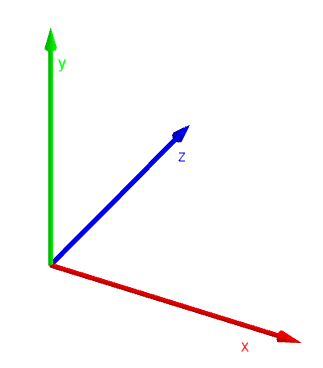
\includegraphics[height=7cm]{unity-axes.png}
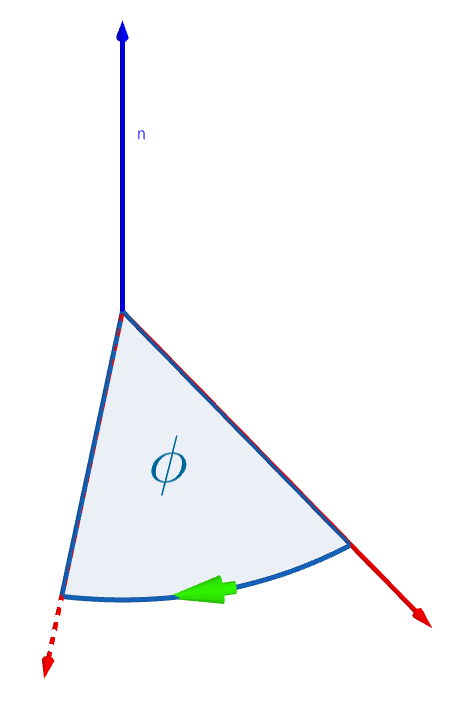
\includegraphics[height=7cm]{unity-rotation.png}
\caption{Unity coordinate system}
\label{fig:unity-coordinate}
\end{figure}

There are several ways to rotate points, vectors or whole transformations. For clarity, let us assume a 3-dimensional vector $\mathbf{u}$ that is to be rotated. We define a rotation unit vector $\mathbf{n}$ and an angle $\phi$ by which we rotate $\mathbf{u}$ so that $\mathbf{u}$ rotates by $\phi$ within a plane to which $\mathbf{n}$ is normal. We also assume that the rotation plane passes through the origin. Then from the perspective of a sundial (with $\mathbf{n}$ being the gnomon) $\mathbf{u}$ rotates \textit{clockwise} for positive $\phi$ (Figure \ref{fig:unity-coordinate}). This holds for all relative rotations.

\subsection{Sectional planes and great circles}
Sphere can have any number of sectional planes, i. e. planes that have some non-empty intersection with the sphere. Planes passing the center of the sphere will be called \textit{sectional central planes} (Figure \ref{fig:sectional-plane}). Any sectional central plane $\rho$ is characterized by some non-zero normal vector $\textbf{n}_\rho$ and for any point on the plane represented by their position vector $\mathbf{x}$ it holds that
$$\mathbf{n}_\rho\cdot\mathbf{x}=0$$
This is synonymous to the fact that any vector lying within a plane passing the origin is perpendicular to the normal vector of the plane. The dot product on the left side of the equality is also important because given a specific normal vector we can decide \textit{on which side} is any vector $\mathbf{x}$ outside the plane -- simply take the sign of the dot product, vector on the side of the normal vector will result in a positive dot product value with $\mathbf{n}_\rho$, negative otherwise.

An important object on the surface of a sphere is a great circle. It is any circle that shares its center and radius with the sphere (Figure \ref{fig:great-circle}). It is also the intersection of a plane passing the center of the sphere with its surface.
\begin{figure}[ht]
\centering
\begin{subfigure}{7cm}
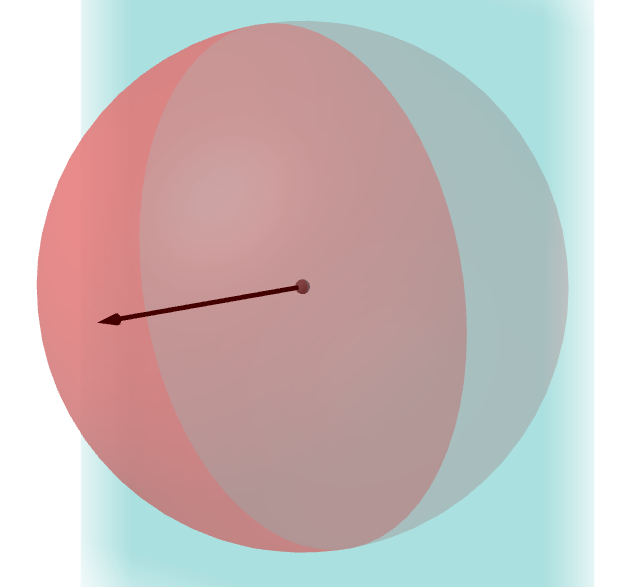
\includegraphics[height=6cm]{sectional-plane.png}
\caption{central plane}
\label{fig:sectional-plane}
\end{subfigure}
\begin{subfigure}{7cm}
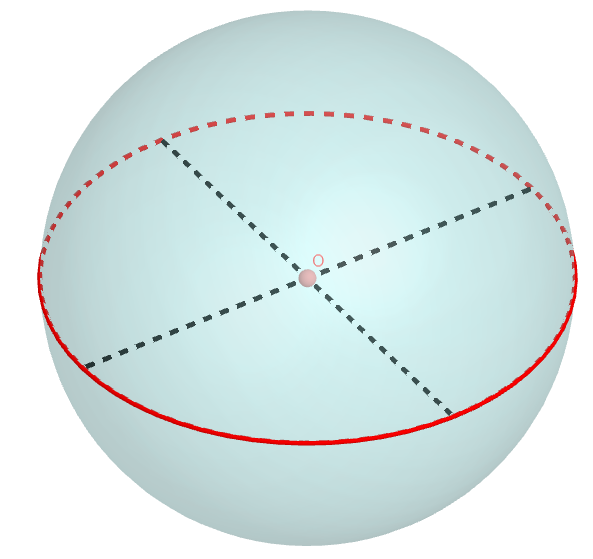
\includegraphics[height=6cm]{great-circle.png}
\caption{great circle}
\label{fig:great-circle}
\end{subfigure}
\caption{Sphere section by plane}
\label{fig:sectional-objects}
\end{figure}

\subsection{Spherical triangles}
\label{subsec:spherical-triangles}
Any three points on the surface of a sphere that do not lie on a single great circle form a~\textit{spherical triangle} (Figure \ref{fig:spherical-triangle}). This is the fundamental concept behind many of the computations in the project. However, strictly speaking, there are two triangles defined by such three points. The closure of the complement of any spherical triangle with respect to the sphere surface is also a spherical triangle, albeit one of the two is unintuitive as it is larger than half of the sphere surface area. To get around this, we construct somewhat narrower class of spherical triangles so that any three valid points define a triangle unambiguously.

\begin{figure}[ht]
\centering
\begin{subfigure}{8cm}
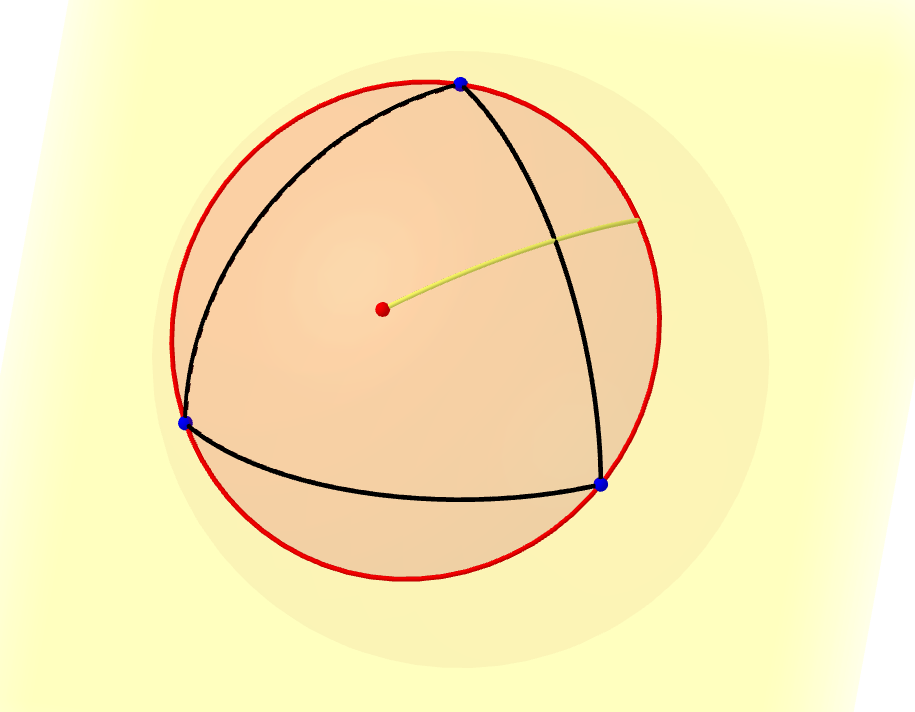
\includegraphics[height=6cm]{triangle-circumcircle.png}
\caption{with sectional plane and circumcircle}
\label{fig:triangle-circumcircle}
\end{subfigure}
\begin{subfigure}{8cm}
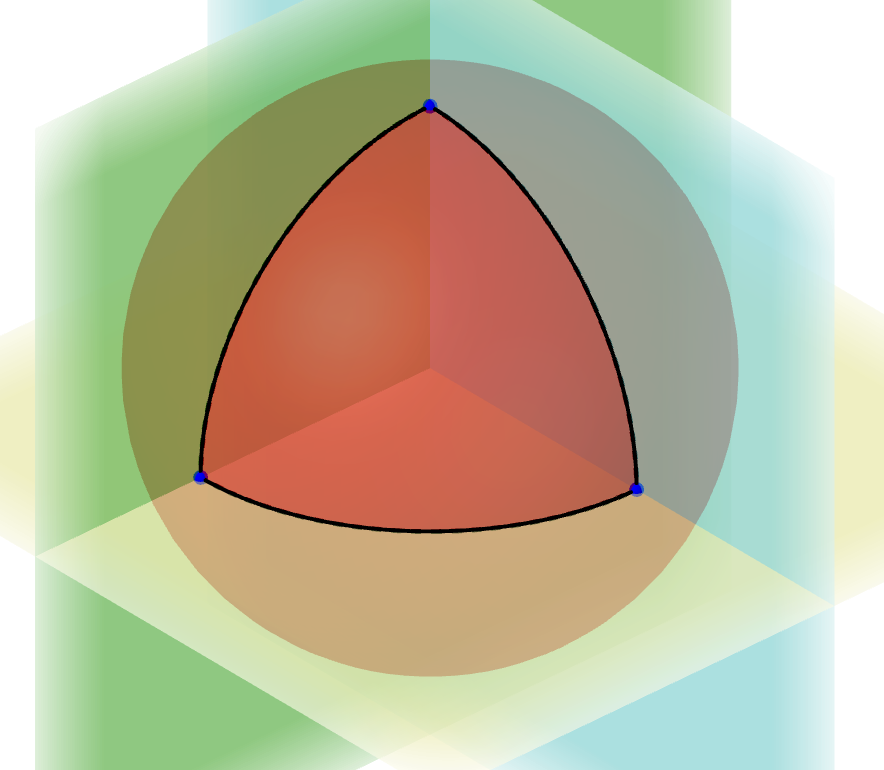
\includegraphics[height=6cm]{triangle.png}
\caption{planes intersections}
\label{fig:spherical-triangle-visual}
\end{subfigure}
\caption{Spherical triangle}
\label{fig:spherical-triangle}
\end{figure}

 We denote the surface of a unit sphere $\mathcal{S} =  \{\mathbf{x} \in \mathbb{R}^3: ||\mathbf{x}||=1\}$. Given a triplet of three linearly independent point vectors $(\mathbf{a},\mathbf{b},\mathbf{c})\in \mathcal{S}\times\mathcal{S}\times\mathcal{S}$ (called \textit{vertices})\footnote{Linear independence of unit vectors is equivalent to the condition that the vectors do not lie on a single great circle.}, we can construct a vector $\mathbf{n}_\lambda$ normal to some sectional plane $\lambda$ cutting off a spherical cap (Figure \ref{fig:triangle-circumcircle}):
 $$\mathbf{n}_\lambda=(\mathbf{b} - \mathbf{a})\times(\mathbf{c} - \mathbf{a})$$
$$\forall\mathbf{x}\in\lambda: \mathbf{n}_\lambda\cdot\mathbf{x}+d_\lambda=0$$
We can calculate $d_\lambda$ by assigning e. g. $\mathbf{x}=\mathbf{a}$ and solving the plane equation with respect to $d_\lambda$, but that will not be neccessary. We impose a further requirement $\mathbf{n}_\lambda\cdot\mathbf{a}>0$. This is not always true, in which case it can be ensured by swapping any two vertices in the triplet and recalculating $\mathbf{n}_\lambda$. This means that all three vertices and their circumcenter are all 'on one side' of the sphere. In Unity coordinate system, this also means that for an outside observer, the vertices are oriented \textit{clockwise} on the sphere surface.

Spherical circumcircle $l$ is a set of points on a sphere that has constant spherical distance from a single point $\mathbf{c}_\mathcal{T}\in\mathcal{S}$ called \textit{circumcenter}. Equivalently, we can substitute dot product for distance:
$$\exists t\in\mathbb{R}:(\forall\mathbf{x}\in l:\mathbf{c}_\mathcal{T}\cdot\mathbf{x}=t)$$
Since $\mathbf{n}_\lambda\cdot\mathbf{a}=\mathbf{n}_\lambda\cdot\mathbf{b}=\mathbf{n}_\lambda\cdot\mathbf{c}>0$, we know that some scalar multiple of $\mathbf{n}_\lambda$ is the circumcenter for the vertices. In fact, there is only one possible circumcircle for all three vertices, which is the intersection $\mathcal{S}\cap\lambda$. We easily find the circumcenter and the circumradius $r_l$ as\footnote{We have to keep in mind that on a unit sphere, central angle and spherical distance are identical, barring formal dimension.}
$$\mathbf{c}_\mathcal{T}=\frac{\mathbf{n}_\lambda}{||\mathbf{n}_\lambda||}, r_l=\arccos(\mathbf{c}_\mathcal{T}\cdot\mathbf{a})$$

Previous reasoning allows us now to test if some point $\mathbf{x}\in\mathcal{S}$ is inside a spherical triangle $\mathcal{T}\subset\mathcal{S}$ with clockwise-oriented vertices $(\mathbf{a}, \mathbf{b}, \mathbf{c})$.
Geometrically speaking, a spherical triangle is a region bounded by three arcs of great circles \cite{palmer}. We calculate three normal vectors:
$$\mathbf{n}_{\rho}=\mathbf{a}\times\mathbf{b},$$
$$\mathbf{n}_{\sigma}=\mathbf{b}\times\mathbf{c},$$
$$\mathbf{n}_{\tau}=\mathbf{c}\times\mathbf{a}.$$
These vectors define planes $\rho, \sigma, \tau$ so that
$$\rho=\{\mathbf{x}\in\mathbb{R}^3:\mathbf{n}_{\rho}\cdot\mathbf{x}=0\}$$
$$\sigma=\{\mathbf{x}\in\mathbb{R}^3:\mathbf{n}_{\sigma}\cdot\mathbf{x}=0\}$$
$$\tau=\{\mathbf{x}\in\mathbb{R}^3:\mathbf{n}_{\tau}\cdot\mathbf{x}=0\}$$
intersections $\rho\cap\mathcal{S}, \sigma\cap\mathcal{S}, \tau\cap\mathcal{S}$ are then great circles that always pass two of the vertices. Because of this, each one is divided by them into two arcs. There is only one triplet of arcs connected by the vertices that forms a meaningful region boundary on $\mathcal{S}$ (Figure \ref{fig:spherical-triangle-visual}). There are two such regions but we already bypassed this problem by ensuring orientation. We test the point $\mathbf{x}$ against following condition:
$$\mathcal{T}=\{\mathbf{x}\in\mathcal{S}:\mathbf{n}_{\rho}\cdot\mathbf{x}\ge 0, \mathbf{n}_{\sigma}\cdot\mathbf{x}\ge 0, \mathbf{n}_{\tau}\cdot\mathbf{x}\ge 0\}$$
This simply tells us that $\mathbf{x}$ is inside the spherical triangle $\mathcal{T}$ when it is on the surface of the sphere and also on one specific side of all three planes $\rho, \sigma, \tau$. This definition does not encompass all possible spherical triangles on a sphere, but it allows us to properly test the properties of any triangles used in reasonable spherical meshes.
\subsection{Vertex sampling}
Because of memory restrictions, sphere surface data is represented as a set of sampled points. We can identify these points as position vectors $\mathbf{u}_i$ from the global origin to sample points, resulting in a~sequence $U=\left(\mathbf{u}_i\right)_{i=0}^{N-1}, \mathbf{u}_i \in \mathcal{S}$. Samples are therefore three-dimensional normalized vectors. Driftworld uses spherical Fibonacci sampling \cite{keinert}. To get the sequence $U$, another sequence $F=\left(\mathbf{f}_i\right)_{i=0}^{N-1}$ is first computed, using the following definition:
$$\mathbf{f}_i=(\phi_i, z_i), \phi_i \in [0,2\pi), z_i \in (-1,1),$$
$$\phi_i = 2\pi\left[\frac{i}{\Phi}\right],$$
$$z_i = 1-\frac{2i+1}{N}.$$
$\left[x\right]$ denotes the fractional part of $x$, $\Phi$ is the golden ratio $\Phi=\frac{\sqrt{5}+1}{2}$. The values of $\mathbf{f}_i$ actually lie on a~spiral on the surface of a cylinder with the radius of 1 and the height of 2 \cite{keinert}. $U$ is finally obtained by mapping $\mathbf{f}_i$ values to $\mathcal{S}$:
$$\mathbf{u}_i = (\sin{(\arccos{(z_i)})}\cdot\cos{\phi_i}, z_i, \sin{(\arccos{(z_i)})}\cdot\sin{\phi_i})$$
Note that this mapping reflects Unity's axes orientation and the first and the last samples of $U$ do not fall exactly on the poles.
\subsection{Centroids, data values and barycentric interpolation}
Driftworld often makes computations for points inside sperical triangles - notably, it uses triangle centroids to evaluate triangle neighbours. Calculating these points is not a trivial procedure and although for a long time there have been methods to do so, it would be too resource-consuming when performed on a larger scale. To save computation time, we assume that all evaluated triangles are nearly planar, i. e. their \textit{triangle excess} is negligible (Legendre's Theorem\footnote{This theorem is also known as Saccheri-Legendre theorem.} \cite{todhunter}). We calculate the centroid of a triangle by simply normalizing the sum of its vertices (Figure \ref{fig:triangle-centroid}):
$$\mathbf{b}_\mathcal{T}=\frac{\mathbf{a} + \mathbf{b} + \mathbf{c}}{||\mathbf{a} + \mathbf{b} + \mathbf{c}||}$$
\begin{figure}[ht]
\centering
\begin{subfigure}{7cm}
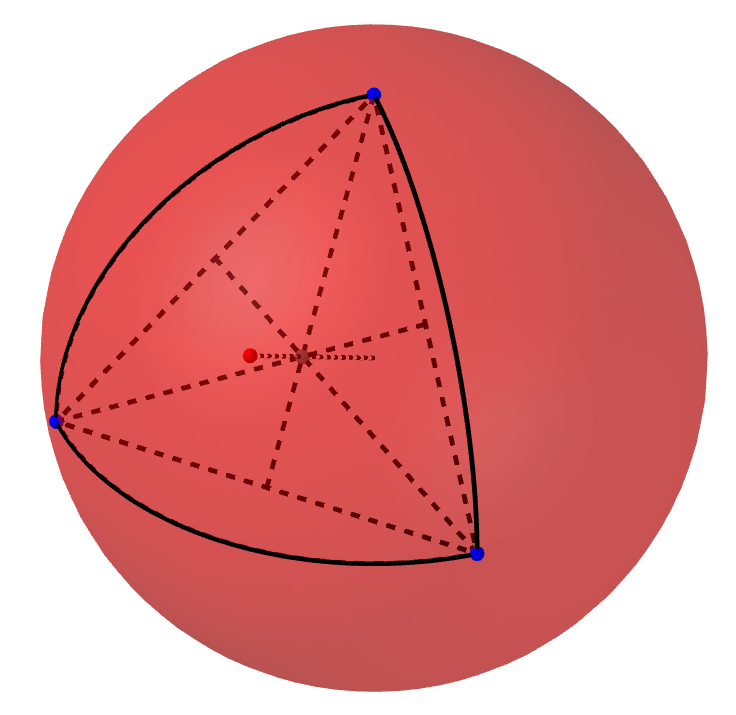
\includegraphics[height=6cm]{triangle-centroid.png}
\caption{sectional triangle centroid}
\label{fig:triangle-centroid}
\end{subfigure}
\hspace*{1cm}
\begin{subfigure}{7cm}
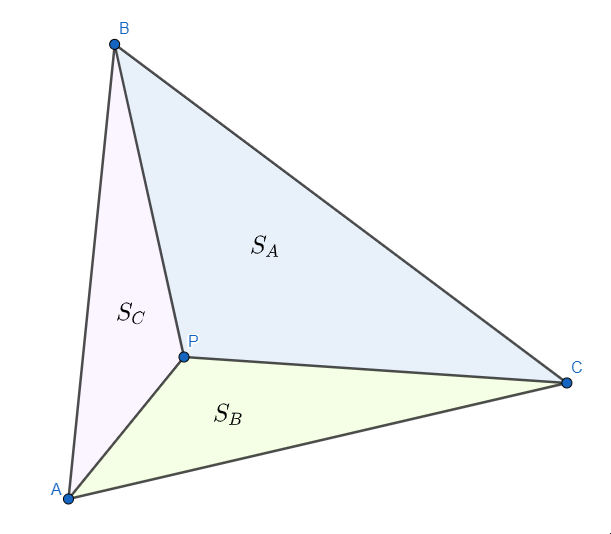
\includegraphics[height=6cm]{triangle-barycentric.png}
\caption{barycentric coordinates}
\label{fig:triangle-barycentric}
\end{subfigure}
\caption{Centroid geometry}
\label{fig:centroid-geometry}
\end{figure}

To store crust data, we must assign values to points on the sphere. These values may be of different types or have different meaning. Formally, we denote a sequence of arbitrary sets $C=\left(V_i\right)_{i=0}^{n-1}$, where $n$ is the number of different values assigned to a point and each $V_i$ is a specific set of possible values. The system of all possible value combinations is then a cartesian product of these value sets:
$$V=\prod_{i=0}^{n-1}V_i$$
Stored data can then be defined as a map:
$$h: U\rightarrow V$$
$$h_i: U\rightarrow V_i$$
We store data only for sphere samples because of limited memory. Other values will be computed as needed using \textit{barycentric interpolation} \cite{scratchapixel}.\newpage

Now it comes to the following problem: how to compute values anywhere on $\mathcal{S}$? We are effectively looking for some domain extension, since $U\subset\mathcal{S}$:
$$h':\mathcal{S}\rightarrow V, \forall \mathbf{u}\in U:h'(\mathbf{u})=h(\mathbf{u})$$
$$h_i':\mathcal{S}\rightarrow V_i, \forall \mathbf{u}\in U:h_i'(\mathbf{u})=h_i(\mathbf{u})$$
Given some arbitrary point $\mathbf{x}\in\mathcal{S}$, we start with an assumption that $\mathbf{x}$ is found inside some spherical triangle $\mathcal{T}$ with negligible triangle excess and vertices $\{\mathbf{a}, \mathbf{b}, \mathbf{c}\} \subset U$ for which we already know the values of $h$. We would like $h'(\mathbf{x})$ to be computed 'fairly', i. e. the closer $\mathbf{x}$ is to some vertex, the more influence the vertex value should have on $h'(\mathbf{x})$. A good start might be in analogy with a political voting system based on area. If the population is homogeneous, any region vote is weighted by its area and transitionally, by its population.

Let $P$ be some point within a triangle $ABC$ (Figure \ref{fig:triangle-barycentric}). This point is represented by a point vector $\mathbf{p}\in\mathcal{S}$. As stated earlier, we assume all points lie nearly on the same plane. If we construct three triangles $PBC$, $APC$ and $APB$, the triangle $ABC$ will be divided into three regions, each corresponding to their oposite vertex of $ABC$. The closer $P$ is to any of the vertices, the larger the corresponding triangle area is. Total area sum of the three triangles is equal to the area of $ABC$. Therefore, we can use these triangle areas as weights for interpolating values at $P$ -- we only need to find the respective areas of $S_A, S_B, S_C$ and $S_{ABC}$. This can be done using cross product:
$$S_A=\frac{|(\mathbf{b}-\mathbf{p})\times(\mathbf{c}-\mathbf{p})|}{2}$$
$$S_B=\frac{|(\mathbf{c}-\mathbf{p})\times(\mathbf{a}-\mathbf{p})|}{2}$$
$$S_C=\frac{|(\mathbf{a}-\mathbf{p})\times(\mathbf{b}-\mathbf{p})|}{2}$$
$$S_{ABC}=\frac{|(\mathbf{b}-\mathbf{a})\times(\mathbf{c}-\mathbf{a})|}{2}$$
Since $S_A+S_B+S_C=S_{ABC}$, we can define normalized weights $u, v, w$ called \textit{barycentric coordinates}:
$$u=\frac{|(\mathbf{b}-\mathbf{p})\times(\mathbf{c}-\mathbf{p})|}{|(\mathbf{b}-\mathbf{a})\times(\mathbf{c}-\mathbf{a})|}$$
$$v=\frac{|(\mathbf{c}-\mathbf{p})\times(\mathbf{a}-\mathbf{p})|}{|(\mathbf{b}-\mathbf{a})\times(\mathbf{c}-\mathbf{a})|}$$
$$w=\frac{|(\mathbf{a}-\mathbf{p})\times(\mathbf{b}-\mathbf{p})|}{|(\mathbf{b}-\mathbf{a})\times(\mathbf{c}-\mathbf{a})|}$$
It is easy to confirm that $u+v+w=1$.

There are basically two types of values interpolated in the project -- real values and categories. Real value interpolation is straightforward:
$$h_i'(\mathbf{p})=uh_i(\mathbf{a})+vh_i(\mathbf{b})+wh_i(\mathbf{c})$$
Categories are simply assigned to $\mathbf{p}$ according to the largest weight:
$$u=\mbox{max}(\{u,v,w\})\Rightarrow h_j'(\mathbf{p})=h_j(\mathbf{a})$$
$$v=\mbox{max}(\{u,v,w\})\Rightarrow h_j'(\mathbf{p})=h_j(\mathbf{b})$$
$$w=\mbox{max}(\{u,v,w\})\Rightarrow h_j'(\mathbf{p})=h_j(\mathbf{c})$$
This effectively draws a Voronoi map according to categories \cite{voronoi}.
\subsection{Spherical mesh and Delaunay triangulation}
There is a basic sphere mesh, provided by Unity (Figure \ref{fig:unity-mesh}). It is like a detailed cubic mesh, projected onto a sphere. However, for finer terrain details, a much more detailed mesh is needed, preferably with uniform triangles (Figure \ref{fig:delaunay-mesh}).

\begin{figure}[ht]
\centering
\begin{subfigure}{7cm}
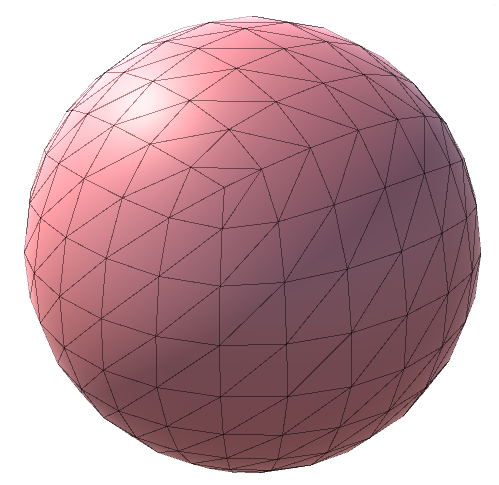
\includegraphics[height=7cm]{unity-mesh.png}
\caption{Unity sphere mesh}
\label{fig:unity-mesh}
\end{subfigure}
\hspace*{1cm}
\begin{subfigure}{7cm}
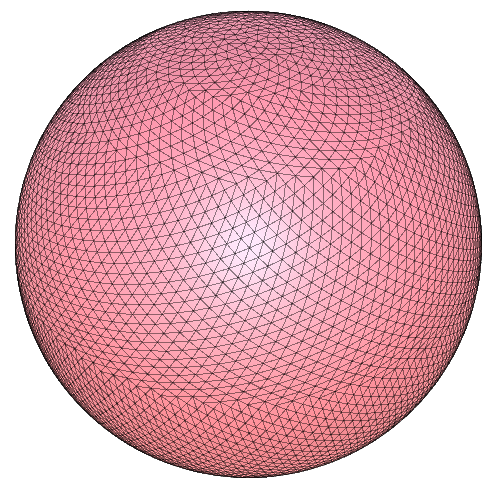
\includegraphics[height=7cm]{delaunay-mesh.png}
\caption{Delaunay mesh}
\label{fig:delaunay-mesh}
\end{subfigure}
\caption{Spherical meshes}
\label{fig:spherical-mesh}
\end{figure}
Definition and description of a 3D mesh is way beyond the scope and purpose of this document. In this context, it is simply an approximation of the sphere surface. All samples $U$ are vertices connected into triangles so that the whole sphere is covered by them without any gaps. For Driftworld, a set of prepared meshes is provided, created by \textit{Delaunay triangulation}\footnote{The triangulation algorithm is not a part of Driftworld. The meshes were actually constructed in a separate tool written in C++ and then added as data files to Driftworld Tectonics repository.} \cite{delaunay}.

When interpolating surface data such as elevation, it is important that reasonable samples are used for the interpolation. Calculating elevation in a mountain range from a triangle with vertices too far apart may result in meaningless artifacts. Furthermore, the earlier mentioned requirement that the triangles are nearly planar would be undermined by extreme spherical triangles which exhibit considerable excess. It stands to reason that triangles used in the mesh should be as regular as possible. This is the goal and result of a Delaunay triangulation. There is a number of algorithms performing the triangulation on a plane \cite{knuth}. Since a sphere has a closed mesh, an adaptation is needed.

Delaunay meshes for Driftworld use an algorithm which originally triangulates a set of random samples \cite{ma}. Because $U$ is ordered, the initial tetrahedron is somewhat difficult to construct, especially because of the requirements imposed on a spherical triangle -- in a large number of cases at least one triangle had a circumcircle larger than a great circle. For this reason, the initial structure was set to be a nearly regular octahedron with vertices assigned by a brute-force look-up. Other than that, the algorithm follows the article \cite{ma}.
\subsection{Collisions}
The tectonic model in Driftworld computes many interactions on a regular basis and these computations must be as efficient as possible. There are two basic collisions used for evaluating interactions -- a collision of two circles and a collision of two triangles. To clarify, in both cases we only need to answer the question whether the two objects have a non-empty intersection -- not to fully classify the intersection. Algorithms for both collisions are fairly simple and the spherical geometry actually helps in the case of triangle collisions.

The relative position of two circles $k,l\subset\mathcal{S}$ is governed by several parameters. Each circle has a~circumcenter $\mathbf{c} \in \mathcal{S}$ and a radius $r > 0$. We consider full circles to determine the intersection:
$$\forall\mathbf{x}\in\mathcal{S}:\arccos(\mathbf{x}\cdot\mathbf{c}_k) \le r_k\Rightarrow\mathbf{x}\in k$$
This means that there is only one case of relative circle position that has an empty intersection: disjoint circles. The case of one circle lying inside another has an intersection indentical to the inside circle. Three major cases of the relative positions of circles are seen in Figure \ref{fig:circle-collisions}.
\begin{figure}[ht]
\centering
\begin{subfigure}{7cm}
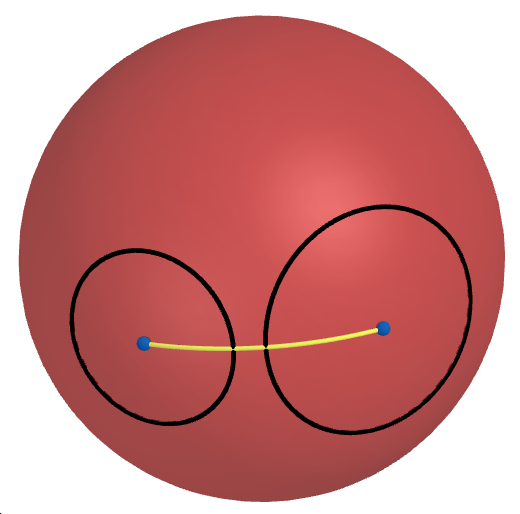
\includegraphics[height=7cm]{circle-intersection-a.png}
\caption{disjoint circles}
\label{fig:disjoint-circles}
\end{subfigure}\\
\begin{subfigure}{7cm}
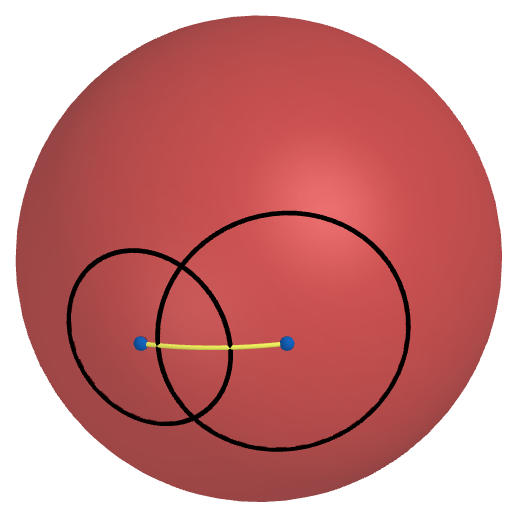
\includegraphics[height=7cm]{circle-intersection-b.png}
\caption{circles intersecting at two points}
\label{fig:circles-intersecting-at-two-points}
\end{subfigure}
\hspace*{1cm}
\begin{subfigure}{7cm}
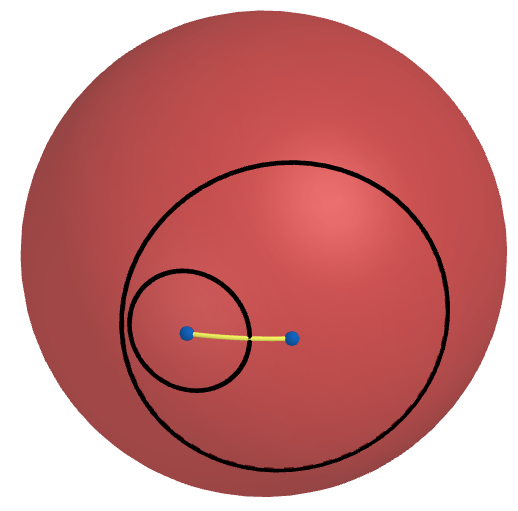
\includegraphics[height=7cm]{circle-intersection-c.png}
\caption{circle lying inside another}
\label{fig:circle-lying-inside-another}
\end{subfigure}
\caption{Relative positions of two circles}
\label{fig:circle-collisions}
\end{figure}

It is therefore easy to decide whether two circles collide or not - circles not colliding have a spherical distance larger than the sum of their radii:
$$k \cap l = \emptyset \Longleftrightarrow \arccos(\mathbf{c}_k\cdot\mathbf{c}_l)>r_k+r_l$$

In case of triangles the collision is more complex. There are four major cases of the relative position of two spherical triangles - three  similar to the case of circles and one specific (see Figure \ref{fig:triangle-collisions}). The second and the third case can be resolved by determining whether any point of one triangle lies within the other (see subsection \ref{subsec:spherical-triangles}). The first and the fourth require a more thorough test.

\begin{figure}[ht]
\centering
\begin{subfigure}{7cm}
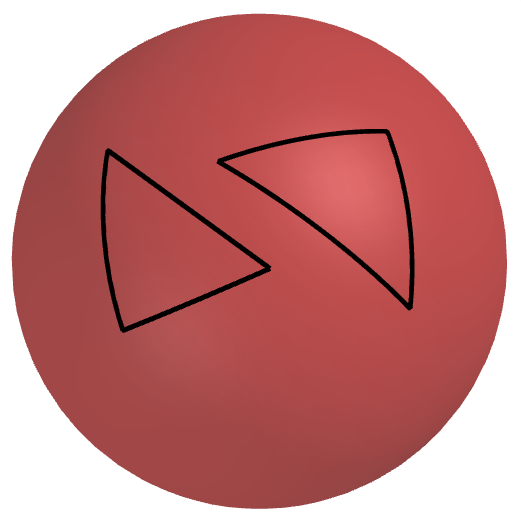
\includegraphics[height=7cm]{triangle-intersection-a.png}
\caption{disjoint triangles}
\label{fig:disjoint-triangles}
\end{subfigure}
\hspace*{1cm}
\begin{subfigure}{7cm}
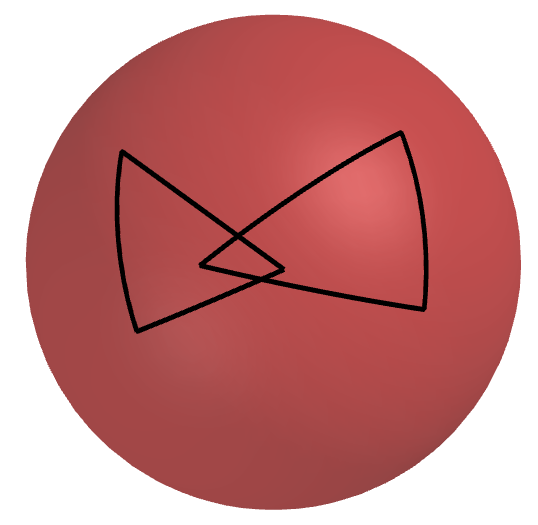
\includegraphics[height=7cm]{triangle-intersection-b.png}
\caption{triangles intersecting at two points}
\label{fig:triangles-intersecting-at-two-points}
\end{subfigure}\\
\begin{subfigure}{7cm}
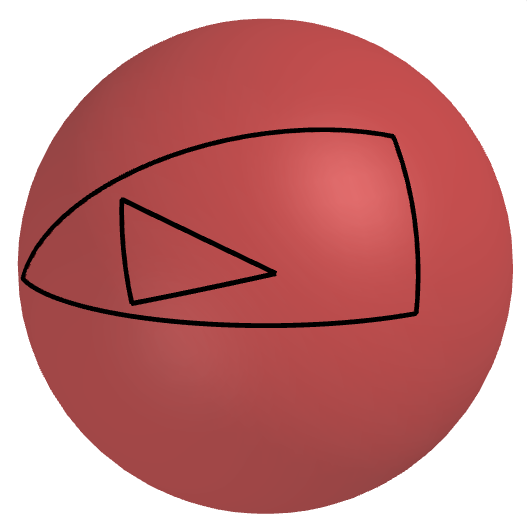
\includegraphics[height=7cm]{triangle-intersection-c.png}
\caption{triangle lying inside another}
\label{fig:triangle-lying-inside-another}
\end{subfigure}
\hspace*{1cm}
\begin{subfigure}{7cm}
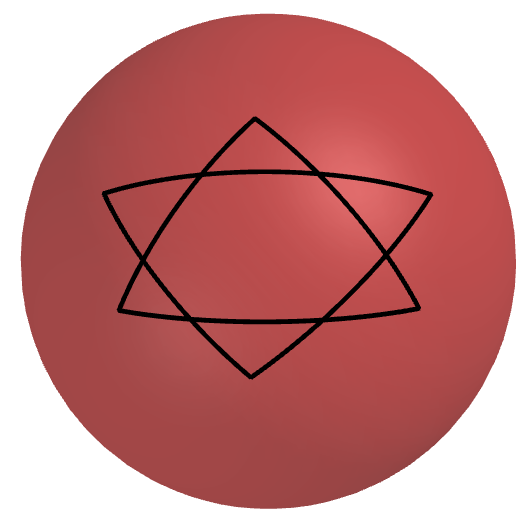
\includegraphics[height=7cm]{triangle-intersection-d.png}
\caption{Star of David}
\label{fig:star-of-david}
\end{subfigure}
\caption{Relative positions of two triangles}
\label{fig:triangle-collisions}
\end{figure}

If neither of the two triangles contain a vertex of the other one, we have to decide if any two edges intersect. Consider two edges defined by pairs of non-identical vertices $(\mathbf{a}_1, \mathbf{a}_2)$ and $(\mathbf{b}_1, \mathbf{b}_2)$. These define planes within which lie their respective great circles. The planes have normal vectors $\mathbf{a}_1 \times \mathbf{a}_2$ and $\mathbf{b}_1 \times \mathbf{b}_2$. Since the planes are central, Any intersection must be along the vector $(\mathbf{a}_1 \times \mathbf{a}_2)\times(\mathbf{b}_1 \times \mathbf{b}_2)$. There are two intersections in $\mathcal{S}$ and we consider the one maximizing the dot product with $\mathbf{a}_1$ (same hemisphere). We denote such intersection $\mathbf{i}$. The final test simply decides if $\mathbf{i}$ lies on both segments or is somewhere else on the great circles. This can be done by testing dot products, as $\mathbf{i}$ must be closer to both vertices than the distance of the vertices for both segments:
$$(\mathbf{i}\cdot\mathbf{a}_1 > \mathbf{a}_1\cdot\mathbf{a}_2) \land (\mathbf{i}\cdot\mathbf{a}_2 > \mathbf{a}_1\cdot\mathbf{a}_2)\land(\mathbf{i}\cdot\mathbf{b}_1 > \mathbf{b}_1\cdot\mathbf{b}_2) \land (\mathbf{i}\cdot\mathbf{b}_2 > \mathbf{b}_1\cdot\mathbf{b}_2)$$
If any two segments of the two triangles intersect, the triangles must by the sign analysis have non-empty intersection and therefore collide. If all tests are negative, the triangles are disjoint.
\subsection{Merging of spherical circles}
Because of the need to build bounding volume hiearchies (see subsection \ref{subsec:bvh}), there is a task of finding a~suitable circle $l$ which has the smallest area possible and which contains two other given circles $m,n$ (see Figure \ref{fig:circles-merged}). The center of $l$ must lie on a great circle $L$ containing both centers of the circles. This means we have to find a center and radius of $l$ so that it only touches either both of the two circles $m,n$ or one in case one circle is within the other. The algorithm falls in at least one of the following cases: concentric circles, circles with opposite centers, one circle contained in the other, circles intersecting at two points or disjoint circles. The goal is to determine which case has the deciding influence on the position of the center $\mathbf{c}_l$ and the radius $r_l$ except in the case of concentric circles, where $l$ is found easily. In case of concentric circles the solution is:
$$\mathbf{c}_l=\mathbf{c}_m, r_l=\mbox{max}(r_m, r_n)$$
Otherwise we find a suitable local basis in which we can easily parametrize all relevant points (Figure \ref{fig:merging-local-basis}). One circle center will be identical to the base vector:
$$\mathbf{e}_x'=\mathbf{c}_m$$
\begin{figure}[ht]
\centering
\begin{subfigure}{7cm}
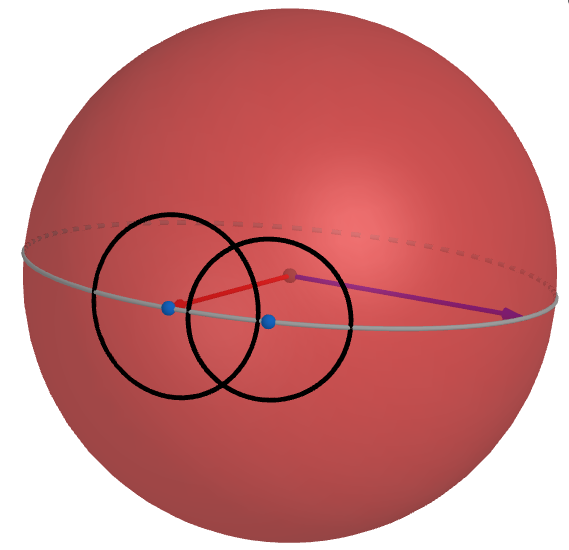
\includegraphics[height=7cm]{merging-local-basis.png}
\caption{local basis}
\label{fig:merging-local-basis}
\end{subfigure}
\hspace*{1cm}
\begin{subfigure}{7cm}
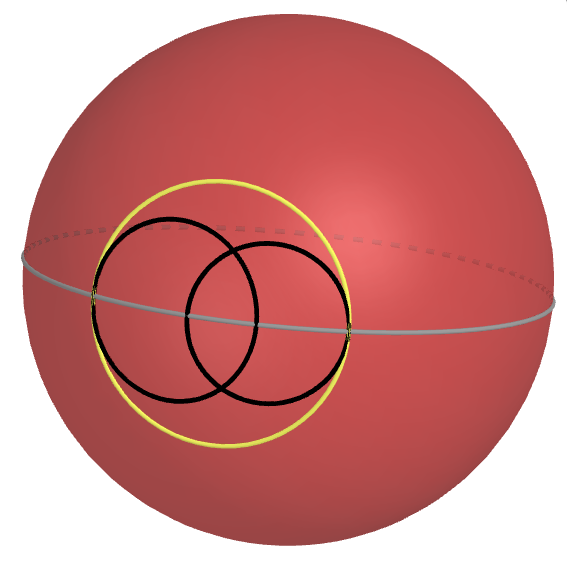
\includegraphics[height=7cm]{circle-joining.png}
\caption{circles merged}
\label{fig:circles-merged}
\end{subfigure}
\caption{Merging of two circles}
\label{fig:merging-circles}
\end{figure}

Computation of the second base vector $\mathbf{e}_z'$ depends on whether the circles are directly opposite, i. e. they have centers opposite on the sphere. If so, it is any vector perpendicular to $\mathbf{e}_x'$ since the centers lie on inifinitely many great circles. If not, it it can be found with a double cross product:
$$\mathbf{e}_z'=\frac{(\mathbf{c}_m\times\mathbf{c}_n)\times\mathbf{c}_m}{||(\mathbf{c}_m\times\mathbf{c}_n)\times\mathbf{c}_m||}$$
There are three variables we need to compute now. First is the distance $d_{mn}$ between $\mathbf{c}_m$ and $\mathbf{c}_n$:
$$d_{mn}=\arccos(\mathbf{c}_m\cdot\mathbf{c}_n)$$
Second is the central angle $\Delta\phi$ of an arc running between $\mathbf{c}_m$ and the center of the merged circle. This allows us to compute the center as a linear combination of the base vectors $(\mathbf{e}_x', \mathbf{e}_z')$. Third is the actual radius $r_l$. However, we first need to see if one of the circles is contained within the other. If so, then one boundary is pushed by the encompassing circle:
$$-r_m > d_{mn} - r_n \Longrightarrow \Delta\phi=d_{mn}, r_l = r_n$$
$$r_m > d_{mn} +  r_n \Longrightarrow \Delta\phi=0, r_l = r_m$$
The first condition is for $n$ encompassing $m$, the second is the other way around. If neither is true, the computation is slightly more difficult:
$$\Delta\phi=\frac{d_{mn}-r_m+r_n}{2}$$
$$r_l=\frac{r_m + r_n + d_{mn}}{2}$$
Finally, we compute the center of $l$\footnote{Note that the value of $\Delta\phi$ can be negative. This is the case of clockwise-oriented arc from $\mathbf{c}_m$ in the local basis.}:
$$\mathbf{c}_l=\cos(\Delta\phi)\mathbf{e}_x' + \sin(\Delta\phi)\mathbf{e}_z'$$
\subsection{Texture mapping}
The system of overlays requires creating a texture every time the planet is to be rendered. Suppose we have a texture with resolution $w\times h$ that should have a color $b_{ij}$ from some color space $\mathcal{C}$ assigned to each of its points:
$$i\in\mathcal{I}=\{0,1,2,...,w-1\}$$
$$j\in\mathcal{J}=\{0,1,2,...,h-1\}$$
$$b:\mathcal{I}\times\mathcal{J}\rightarrow\mathcal{C}$$
We want $b_{ij}$ to reflect the data on the sphere. Let $b'$ be a map from the sphere surface, representing an overlay:
$$b': \mathcal{S}\rightarrow\mathcal{C}$$
We now have to find some map between the pixel indices and the sphere surface. This is very similar to the classical problem in cartography. Our choice will be an equirectangular projection because of its simplicity. We first compute the azimuthal and polar angles $\phi_i, \theta_j$ from $i,j$:
$$\phi_i = 2\pi\frac{\left(i+\frac{1}{2}\right)}{w}$$
$$\theta_j = \pi(1-\frac{j+\frac{1}{2}}{h})$$
\begin{figure}[ht]
\centering
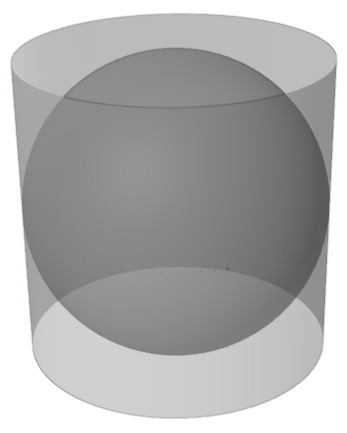
\includegraphics[height=7cm]{texture-coordinates.png}
\caption{Cylinder rectangle around a sphere}
\label{fig:rectangle-sphere}
\end{figure}
This means the texture $y$ coordinate increases \textit{upwards} (to north) in the respective cylinder rectangle (Figure \ref{fig:rectangle-sphere}). From the angles it is simple to find the point on the sphere:
$$\mathbf{x}_{ij} = (\sin\theta_j\cos\phi_i,\cos\theta_j,\sin\theta_j\sin\phi_i)$$
Finally, we can compute $b_{ij}$:
$$b_{ij}=b'(\sin\theta_j\cos\phi_i,\cos\theta_j,\sin\theta_j\sin\phi_i)$$
This texture is subsequently used for rendering the surface, however, there is an inherent problem with uv mapping. Because of my insecurity about the math involved, the process will not be explained in this text and instead, the reader is encouraged to read a more educated article \cite{bgolus}.

There is perhaps a better way to deal with texture mapping, which was discussed in a Unity forum thread \cite{unityforum}. Cubemaps are quite possibly a more logical choice, as the texture information density needlesly increases towards extreme values of the $y$ coordinate.
\subsection{Unit dimensions}
Virtually all expressions throughout this section assumed a unit sphere for simplicity, but for rendering and parameter context some scaling is needed. For example, radius $R$ of the planet might be given in kilometers \cite{cortial}. Quantities such as this one describe planets in a~physical metric space with a~basic length unit of 1 m (and its metric prefixes). We consider the basic length unit in Unity scenes a 'Unity meter' $\mbox{u}$ and the corresponding space as Unity space. Given standard radius of a planet (in order of 1000 km), rendering in 1:1 scale from metric to Unity space is impractical. We set a scale convention $1\mbox{ u}=1000\mbox{ km}$. Because of the geological time scale, our basic unit of time will be $\mbox{My}$ (million years). Some useful conversions follow in table \ref{tab:unit-conversion}.

The planet radius expressed in Unity meters is used as a scaling parameter to transform quantities from Unity space to the unit sphere representation (denoted by $R_\mathcal{U}$). The simulation runs in the unit sphere representation and planet is rendered by scaling the vertices on the unit sphere by $R_\mathcal{U}$.

\paragraph{Example}Planet with a radius $R=6370$ km has a maximum plate speed\footnote{Because Driftworld Tectonics uses the unit sphere values, we will reference quantities declared in the original article~\cite{cortial} as primed.} $v_0'$ of 100 mm$\cdot$y$^{-1}$ and an average plate area $\mathcal{A}_0'$ of $25.5\times 10^{6}\mbox{ km}^2$ . We want to transform these values to a unit sphere representation. The scaling parameter is  $R_\mathcal{U}=6.37$ u. Maximum plate speed is transformed as:
$$v_0 = \frac{v_0'}{R_\mathcal{U}} =  \frac{100\mbox{ mm}\cdot\mbox{y}^{-1}}{6370\mbox{ km}}=\frac{0.1\mbox{ u}\cdot\mbox{My}^{-1}}{6.37\mbox{ u}}\approx 0.0157\mbox{ My}^{-1}$$
This allows us to identify any surface speed with an angular speed. The average area has two length dimensions, so to transform to a unit sphere, the expression is:
$$\mathcal{A}_0 = \frac{\mathcal{A}_0'}{R_\mathcal{U}^2} =  \frac{25.5\times 10^{6}\mbox{ km}^2}{40576900\mbox{ km}^2}= \frac{25.5\mbox{ u}^2}{40.5769\mbox{ u}^2}\approx 0.628$$
Note that the value is fraction-scaled to $4\pi$, which is the unit sphere surface area.
\begin{table}
\centering
\begin{tabular}{rr}
\textbf{Metric unit}&\textbf{Unity conversion}\\
\hline\\
1 km&0.001 u\\
1 km$^{-1}$&1000 u$^{-1}$\\
1 mm$\cdot$y$^{-1}$&$10^{-3}$ u$\cdot$My$^{-1}$
\end{tabular}
\caption{Unit conversion table}
\label{tab:unit-conversion}
\end{table}
\subsection{Vector noise on mesh}
\label{subsec:vector-noise-on-mesh}
Given a Delauney triangulation of a sphere, Driftworld uses a specific type of noise to randomize simple linear borders, such as between two tectonic plates. Because only whole mesh triangles are assigned to plates, a single noise value is assigned to each triangle. Because the goal of the randomizer is to shift border directions, the noise values are vectors. A single value $\mathbf{m}$ is obtained by taking a~random vector $\mathbf{s}\in\mathcal{S}$ and projecting it onto the tangent plane of the triangle centroid $\mathbf{c}$\footnote{This part is similar to the grid vector assignment when calculating 2D Perlin noise \cite{perlinnoise}, although with additional projection.}:
$$\mathbf{m} = \mathbf{s}-(\mathbf{s}\cdot\mathbf{c})\mathbf{c}$$
This way, the obtained random vectors should be uniformly distributed. Note that the vector lengths are from the interval $[0,1]$ and completely random. To avoid some of the border jitter, the noise should be low-frequency. Every triangle has three neighbours along its edges. This means that for every triangle we can average its noise vector with the neighbour noise vectors to filter higher frequency noise. We only need to ensure that the result is again within the tangent plane by projecting either the contributing vectors or the result itself. This summation can be repeated several time to adjust the filtering. 

The resulting low-frequency vector noise is driven by the number of averaging iterations. This is basically a 'smearing' of the triangle noise up to a certain radius. The total number of triangles in a~mesh influences the resulting noise pattern (detail) on the sphere. In Figure \ref{fig:vector-noise} the same number of iterations were used for meshes with 10,000 (\ref{fig:vector-noise-lowpoly}) and 500,000 (\ref{fig:vector-noise-highpoly}) triangles. Hue represents relative direction, saturation the length of a~vector and value is set to constant 1. It is clearly seen that the the granulation is finer on the sphere with more detailed mesh. Also, there is a noise pattern change along the lines where the mesh pattern changes. This is partially because each triangle is colored whole with a single color and the triangles are not perfectly regular.

It might be a good idea to revisit the concept of a vector noise on the sphere some time in the future. The concept is experimental and it is unclear if it has some unforeseen consequences for the plate border interactions.
\begin{figure}[ht]
\centering
\begin{subfigure}{7cm}
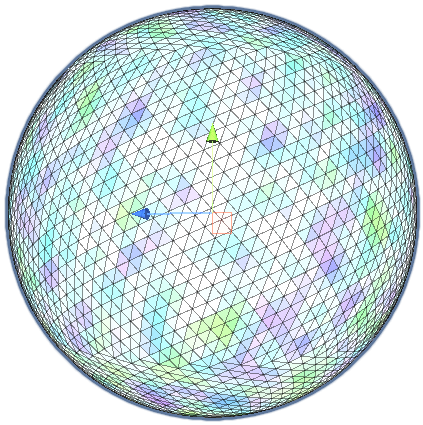
\includegraphics[height=7cm]{vector-noise-lowpoly.png}
\caption{low poly with mesh - whole triangles are coloured}
\label{fig:vector-noise-lowpoly}
\end{subfigure}
\hspace*{1cm}
\begin{subfigure}{7cm}
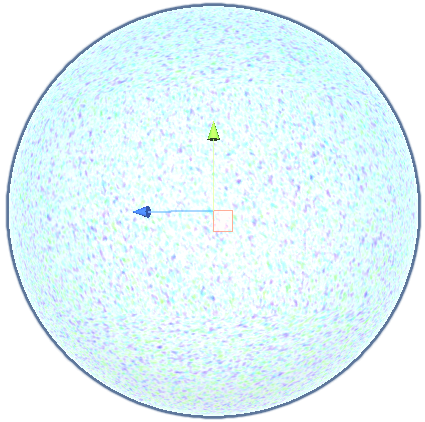
\includegraphics[height=7cm]{vector-noise-highpoly.png}
\caption{high poly without mesh - borders of mesh patterns visible}
\label{fig:vector-noise-highpoly}
\end{subfigure}
\caption{Vector noise representation}
\label{fig:vector-noise}
\end{figure}
\subsection{Elevation Laplacian}
Sometimes it is important to see where some $s_i$ values of mesh points differ in a~significant manner relative to their neighbouring mesh vertices. Driftworld uses this diagnostic method for the elevation values. Let $\mathbf{u}$ be a point on the mesh and $W=\{\mathbf{u}_1,\mathbf{u}_2,\mathbf{u}_3,...,\mathbf{u}_n\}$ a~set of its neighbours along the edges of mesh triangles. Then for some data map $h_j$ we define the mesh point Laplacian as \cite{diffoperators}:
$$L_j(\mathbf{u})=\sum_{i=1}^n\left(h_j(\mathbf{u}_i)-h_j(\mathbf{u})\right)$$
Note that this operation only makes sense for real number values, not categories.
